\documentclass[10pt]{article}
\usepackage{amsmath} 
\usepackage{graphicx}

\begin{document}

\section*{Problema 1: Campo medio}

\begin{equation}
H = -J_2 \sum_{\langle i,j\rangle} \sigma_i \sigma_j - J_4 \sum_I \sigma_{I1}\sigma_{I2}\sigma_{I3}\sigma_{I4}
\end{equation}

Proponemos el hamiltoniano de prueba de spines no interactuantes

\begin{equation}
H_0 = -\eta \sum_i \sigma_i
\end{equation}

y utilizamos la desigualdad de Bogoliuvob-Peierls:

\begin{equation}
f \leq f_{\rho} = f_0 + \dfrac{1}{N} \langle H - H_0 \rangle_0.
\end{equation}

Calculamos la funci\'on de partici\'on para el hamiltoniano de prueba:

\begin{align}
\mathcal{Z}_0 &= \sum_{\lbrace s_i\rbrace} e^{-\beta H_0} \nonumber \\
&= \sum_{\lbrace s_i\rbrace} \exp \left[ \beta \eta \sum_i s_i  \right] \nonumber \\
&= \sum_{\lbrace s_i\rbrace} \prod_i  e^{\beta \eta s_i} \nonumber \\
&= \prod_i \sum_{s_i=\pm1} e^{\beta \eta s_i}  \nonumber \\
&= \left[ e^{-\beta \eta} + e^{\beta \eta} \right]^N \nonumber \\
&= \left[ 2 \cosh\left(\beta \eta\right) \right]^N \nonumber \\
&= \mathcal{Z}_{01}^N,
\end{align}

donde 

\begin{equation}
\mathcal{Z}_{01} = 2 \cosh\left(\beta \eta\right).
\end{equation}

La energ\'ia libre asociada al hamiltoniano de prueba es entonces

\begin{align}
f_0 &= -\dfrac{1}{\beta N} \ln \mathcal{Z}_0 \nonumber \\
&= -\dfrac{1}{\beta} \ln \left[ 2 \cosh\left(\beta \eta\right) \right]
\end{align}

Calculamos la magnetizaci\'on:

\begin{align} \label{eq:BC_m0}
m_0 &= \langle s_i \rangle_0 \nonumber \\
&= \dfrac{1}{\mathcal{Z}_{01}} \sum_{s_i=\pm1} s_i e^{\beta \eta s_i} \nonumber \\
&= \dfrac{1}{\mathcal{Z}_{01}} \left[-e^{-\beta \eta} + e^{\beta \eta} \right] \nonumber \\
&= \tanh\left( \beta \eta \right)
\end{align}


Valores medios de los hamiltonianos respecto del hamiltoniano de prueba:

\begin{align}
\langle H_0 \rangle_0 &= -\eta \sum_i \langle s_i \rangle_0  \nonumber \\
&= -\eta N m_0. \\
\nonumber \\
\langle H \rangle_0 &= -J_2 \sum_{\langle i,j\rangle} \langle s_i s_j \rangle_0 - J_4 \sum_I \langle\sigma_{I1}\sigma_{I2}\sigma_{I3}\sigma_{I4} \rangle_0 \nonumber \\
&= -J_2 \sum_{\langle i,j\rangle} \langle s_i\rangle_0^4 - J_4 \sum_I \langle\sigma_{I1}\rangle_0^4  \nonumber \\
&= -2 J_2 N m_0^2 - J_4 N m_0^4 .
\end{align}

Proponemos la funci\'on variacional 

\begin{align} \label{eq:BC_Phi}
\Phi(\eta) &= f_0 + \dfrac{1}{N} \langle H - H_0 \rangle_0 \nonumber \\
&= -\dfrac{1}{\beta} \ln \left[2 \cosh\left(\beta \eta\right) \right] -2 J_2 m_0^2 - J_4 m_0^4 + \eta m_0
\end{align}

La energ\'ia libre en la aproximaci\'on de campo medio est\'a dada por la expresi\'on que minimiza la funci\'on $\Phi(\eta)$ con respecto a $\eta$. Es decir,

\begin{equation}
f_{\mathrm{mf}}(T,B) = \min_{\eta} \Phi(\eta).
\end{equation}

Derivamos con respecto a $\eta$ e igualamos a cero para hallar el m\'inimo

\begin{align}
\dfrac{\partial \Phi}{\partial \eta} &= - \tanh\left(\beta \eta\right) - 4 J_2 m_0 \dfrac{\partial m_0}{\partial \eta} - 4 J_4 m_0^3 \dfrac{\partial m_0}{\partial \eta} + m_0 + \eta \dfrac{\partial m_0}{\partial \eta} \nonumber \\
&= \left(\eta - 4 J_2 m_0 - 4 J_4 m_0^3\right) \dfrac{\partial m_0}{\partial \eta},
\end{align}

donde usamos la igualdad \ref{eq:BC_m0}.

La expresi\'on anterior implica que la soluci\'on al problema variacional es 

\begin{equation}\label{eq:eta}
\eta = 4 J_2 m_0 + 4 J_4 m_0^3.
\end{equation}

Reemplazando el valor de $\eta$ en \ref{eq:BC_m0}, obtenemos la ecuaci\'on de estado a campo nulo

\begin{equation}
m_0 = \tanh\left[\beta (4 J_2 m_0 + 4 J_4 m_0^3)\right].
\end{equation}

Para simplificar notaci\'on en el resto del desarrollo, definimos las variables $\tilde{\beta} \equiv 4 J_2 \beta$ y $J \equiv J_4/J_2$. De este modo, la ecuaci\'on anterior queda

\begin{equation}
m_0 = \tanh\left[\tilde{\beta} (m_0 + J m_0^3)\right].
\end{equation}



Utilizando  \ref{eq:BC_Phi} y \ref{eq:eta}, tenemos

\begin{equation}
f_{\mathrm{mf}}(T,B=0) = -\dfrac{1}{\beta} \ln \left[2 \cosh\left(\beta ( 4 J_2 m_0 + 4 J_4 m_0^3)\right) \right] +2 J_2 m_0^2 + 3 J_4 m_0^4.
\end{equation}

Reescalamos la energ\'ia en unidades de $J_2$, definiendo $\tilde{f}_{\mathrm{mf}} \equiv f_{\mathrm{mf}}/J_2$. As\'i obtenemos

\begin{equation}
\tilde{f}_{\mathrm{mf}}(T,B=0) = -4\tilde{\beta}^{-1} \ln \left[2 \cosh\left(\tilde{\beta} ( m_0 + J m_0^3)\right) \right] +2 m_0^2 + 3 J m_0^4.
\end{equation}

Haciendo un desarrollo de Taylor a orden 6,

\begin{align}
\tilde{f}_{\mathrm{mf}}(T,B=0) =& \;a_0 + 2(1-\tilde{\beta}) m_0^2 + 
\left(3J - 4J\tilde{\beta} + \dfrac{\tilde{\beta}^3}{3} \right) m_0^4 \nonumber \\
&+ \left(-2 J^2\tilde{\beta} + \dfrac{4J\tilde{\beta}^3}{3} - \dfrac{4\tilde{\beta}^5}{45}\right) m_0^6 + \mathcal{O}(m_0^8)
\end{align}

donde $a_0 = -4\ln(2)/\tilde{\beta}$ es un t\'ermino aditivo que resulta irrelevante. Vemos entonces que la energ\'ia libre queda expresada en forma de funci\'on de Landau

\begin{align}
\tilde{f}_{\mathrm{mf}}(T,B=0) = a_0 + \dfrac{a_2}{2} m_0^2 + 
\dfrac{a_4}{4} m_0^4 + \dfrac{a_6}{6} m_0^6 + \mathcal{O}(m_0^8),
\end{align}

con coeficientes 

\begin{align*}
a_2(T,J) &= 4 (1-\tilde{\beta})\\
a_4(T,J) &= 4\left( 3J - 4J\tilde{\beta} + \dfrac{\tilde{\beta}^3}{3} \right) \\
a_6(T,J) &= 6 \left(-2 J^2\tilde{\beta} + \dfrac{4J\tilde{\beta}^3}{3} - \dfrac{4\tilde{\beta}^5}{45}\right)
\end{align*}

Para construir el diagrama de fases, comencemos analizando si existe transici\'on de segundo orden. La l\'inea de segundo orden se obtiene cuando $a_2=0$ y $a_4>0$. De la primera condici\'on, obtenemos que $\tilde{\beta}_c = 1$, mientras que de la segunda,


\begin{equation}
J < \dfrac{\tilde{\beta}_c^3}{3(4\tilde{\beta}_c-3)}=\dfrac{1}{3}.
\end{equation}

De la definici\'on de $\tilde{\beta}$, se deduce que $k_B T/J_2 = 4 /\tilde{\beta}$, por lo que la temperatura cr\'itica satisface $k_B T_c/J_2 = 4$. La l\'inea de segundo orden se muestra como l\'inea s\'olida en el gr\'afico de la figura \ref{fig:fases}.

La l\'inea de segundo orden termina en el punto tricr\'itico, el cual se ubica en $(\tilde{\beta}_t, J_t)=(1, 1/3)$. A partir de all\'i, comienza la l\'inea de primer orden, que consiste en los puntos $(\tilde{\beta}, J)$ que satisfacen 

\begin{equation}
a_4(T, J)=-\dfrac{\sqrt{a_2(T,J)\;a_6(T,J)}}{3},
\end{equation}

junto con las condiciones $a_2>0$ y $a_6>0$. La l\'inea punteada de la figura \ref{fig:fases} representa la l\'inea de primer orden.

\begin{figure}
\centering
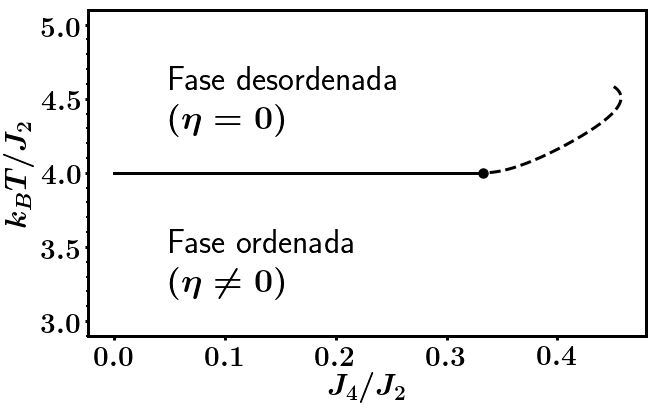
\includegraphics[scale=0.5]{phase_diagram.png}
\caption{\label{fig:fases} Diagrama de fases.}
\end{figure}


\section*{Problema 2: Grupo de renormalizaci\'on}

El hamiltoniando (reducido) de Ising es

\begin{equation}
\mathcal{H} = K \sum_{\langle i, j\rangle} s_i s_j + h \sum_i s_i.
\end{equation}

Renormalizamos utilizando bloques de Kadanoff cuadrados de 4 sitios. La regla de la mayor\'ia puede expresarse como

\begin{equation}
P(s', s) = \prod_I P_I(s',s),
\end{equation}

donde 

\begin{equation}
P_I(s', s) = \dfrac{1}{2} \left[ 1 + S'_I\; \mathrm{sgn}(S_1^I+S_2^I+S_3^I+S_4^I) \right].
\end{equation}

Podemos ver que, en el caso de empate, la expresi\'on anterior asigna la misma probabilidad a cada uno de los dos posibles valores del spin de bloque.

Descomponemos nuestro hamiltoniano en la forma

\begin{equation}
\mathcal{H}(s) = \mathcal{H}_0(s) + \mathcal{V}_0(s),
\end{equation}

donde $\mathcal{H}_0(s)$ es una componente sim\'etrica, con interacciones internas de cada bloque y $ \mathcal{V}_0(s)$  es una componente no sim\'etrica, que incluye las interacciones entre bloques

La funci\'on de partici\'on interna puede expresarse como

\begin{align}
\mathcal{Z}_0^I &= 1\times e^{4K} + 1\times 4 + \dfrac{1}{2}\times 4 + \dfrac{1}{2}\times 2e^{-4K} \nonumber \\
&= e^{4K} + 6 + e^{-4K} \nonumber \\
&= 2 \cosh(4K) + 6
\end{align}

Como todos los spines del bloque son equivalentes, el promedio de spin de sitio es 

\begin{align}
\langle S_i^I \rangle_0 &= \dfrac{1}{\mathcal{Z}_0} \sum_{\lbrace s \rbrace} P(S, s) e^{\mathcal{H}_0}(s) S_i^I \nonumber \\
 &= \dfrac{e^{4K} + 2}{\mathcal{Z}_0^I} S'_I\nonumber \\
&= a(K) S'_I,
\end{align}

donde

\begin{equation}
a(K) =   \dfrac{e^{4K} + 2}{2 \cosh(4K) + 6}.
\end{equation}

El promedio del t\'ermino no sim\'etrico es

\begin{align}
\langle \mathcal{V}(s)\rangle_0 &= K\sum_{\langle I,J\rangle} \langle V_{IJ} \rangle_0 + 4 h \sum_I \langle S_i^I \rangle_0,
\end{align}

donde 

\begin{equation}
V_{IJ} = \sum_{\substack{\langle I,J\rangle/\\ i\epsilon I,j\epsilon J}} S_i S_j.
\end{equation}

En el caso de bloques cuadrados de 4 sitios,

\begin{equation}
V_{IJ} = S_1^I S_4^J+  S_2^I S_3^J.
\end{equation}

Luego,

\begin{equation}
\langle V_{IJ}\rangle_0 = 2\langle S_i^I \rangle_0 \langle S_i^J \rangle_0.
\end{equation}

Entonces,


\begin{align}
\langle \mathcal{V}(s)\rangle_0 &= 2K\sum_{\langle I,J\rangle} \langle S_i^I \rangle_0 \langle S_i^J \rangle_0 + 4 h \sum_I  \langle S_i^I \rangle_0 \nonumber \\
&= 2K a^2(K) \sum_{\langle I,J\rangle} S^I S^J +   4 a(K) h \sum_I S^I 
\end{align}

Las ecuaciones de renormalizaci\'on son entonces

\begin{align}
K' &= 2K\;a^2(K) \\
h' &= 4h\;a(K) 
\end{align}

Calculamos $K^*$ en el subespacio invariante $h=0$:

\begin{align}
a^2(K^*) &= \dfrac{1}{2} \\
e^{4K} + 2 &= \dfrac{\sqrt{2}}{2} \bigg( 2\cosh(4K) + 6 \bigg)
\end{align}

Definimos $u \equiv e^{4K}$, entonces

\begin{align}
u + 2 &= \dfrac{\sqrt{2}}{2} \bigg( u + u^{-1} + 6 \bigg) \\
\left(1 - \dfrac{\sqrt{2}}{2}\right) u^2 + \left(2 - 3\sqrt{2}\right) u - \dfrac{\sqrt{2}}{2}&= 0
\end{align}

La \'unica soluci\'on f\'isica (con $u>1$) es $u^* = 1+2\sqrt{2}+\sqrt{5(2+\sqrt{2})}$. Luego, 

\begin{equation}
K^* = \dfrac{\log{\left[1+2\sqrt{2}+\sqrt{5(2+\sqrt{2})}\right]}}{4} \simeq 0.5186.
\end{equation}

Por las relaciones de paridad, la matriz jacobiana es diagonal e igual a 

$$
\mathcal{L}_b = 
\begin{pmatrix}
b^{y_T} & 0 \\
0 & b^{y_B}
\end{pmatrix},
$$

donde

\begin{align}
b^{y_T} &= \left( \dfrac{\partial K'}{\partial K} \right)_{K^{*},h=0} = 2a^2(K^*)+4K^*a(K^*) a'(K^*) \\
b^{y_B} &= \left( \dfrac{\partial h'}{\partial h} \right)_{K^{*},h=0} = 4a(K^*)
\end{align}

Despejando y evaluando en $K^*$, y teniendo en cuenta que $b=2$, tenemos

\begin{align}
y_T &= \dfrac{\log\left[ \left( \dfrac{\partial K'}{\partial K}  \right)_{K^{*},h=0} \right]}{\log(b)} = 1.006 \\
y_B &= \dfrac{\log\left[ \left( \dfrac{\partial h'}{\partial h}  \right)_{K^{*},h=0} \right]}{\log(b)} = 3/2
\end{align}

Una vez obtenidos los exponentes $y_T$ y $y_B$, todos los dem\'as exponentes se pueden calcular utilizando las relaciones entre exponentes

\begin{align}
\nu &= \dfrac{1}{y_T} =0.9941\\
\alpha &= \dfrac{2d y_T - 1}{y_T} = 0.0117 \\
\beta &= \dfrac{d-y_B}{y_T} = 0.4971 \\
\gamma &= \dfrac{2 y_B - d}{y_T} = 0.9941 \\
\delta &= \dfrac{y_B}{d-y_B} = 3 
\end{align}


\end{document}
